\documentclass[tikz,border=3.14mm]{standalone}
\usepackage{amsmath}

\begin{document}
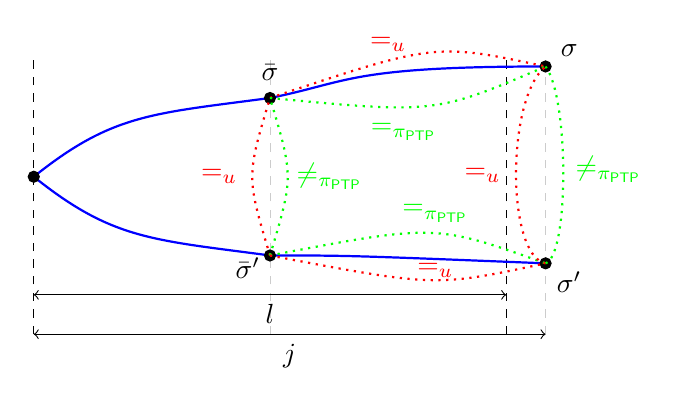
\begin{tikzpicture}
    % Define lengths
    \def\lc{3} % Length of lc
    \def\ls{3} % Length of ls

    % Draw vertical dashed lines (was horizontal in vertical version)
    \draw[dashed] (0,-1) -- (0,2.5);
    \draw[dashed,ultra thin, opacity = 0.2] (\lc, -1) -- (\lc, 2.5);
    \draw[dashed] (\lc+\ls, -1) -- (\lc+\ls, 2.5);
    \draw[dashed, ultra thin, opacity = 0.2] (\lc+\ls+0.5, -1) -- (\lc+\ls+0.5, 2.5);

    % Draw horizontal lines for lc and ls (was vertical in vertical version)
    \draw[<->] (0, -0.5) -- (\lc+\ls, -0.5) node[midway, below] {$l$};
    \draw[<->] (0, -1) -- (\lc+\ls+0.5, -1) node[midway, below] {$j$};

    % Draw curves
    \draw[thick,blue] (0,1) .. controls (\lc/3,1.8) and (\lc/2,1.8) .. (\lc,2)
        .. controls (\lc+\ls/3,2.2) and (\lc+\ls/3,2.4) .. (\lc+\ls+0.5,2.4) node[right] {};

'

    \draw[thick,blue] (0,1) .. controls (\lc/3,0.2) and (\lc/2,0.2) .. (\lc,0)
        .. controls (\lc+\ls/3,-0) and (\lc+\ls/3,-0) .. (\lc+\ls+0.5,-0.1) node[right] {};

    % Add points
    \filldraw (0,1) circle (2pt);
    \filldraw (\lc,2) circle (2pt);
    \filldraw (\lc,0) circle (2pt);
    \filldraw (\lc+\ls+0.5,2.4) circle (2pt);
    \filldraw (\lc+\ls+0.5,-0.1) circle (2pt);

    % Add labels for points
    \node[above] at (\lc,2.1) {$\bar{\sigma}$};
    \node[below left] at (\lc,0.1) {$\bar{\sigma}'$};

    % Add labels
    \node[above] at (\lc+\ls+0.8,2.4) {$\sigma$};
    \node[above] at (\lc+\ls+0.8,-0.6) {$\sigma'$};

    % Draw dashed parallel curves from \bar{\sigma} and \bar{\sigma'}

    % Draw red curve connecting \bar{\sigma} to \bar{\sigma'}
    \draw[red,dotted,thick] (\lc,-0) .. controls (\lc-0.3,1) and (\lc-0.3,1) .. (\lc,2);

    \draw[green,dotted,thick] (\lc,0) .. controls (\lc+0.3,1) and (\lc+0.3,1) .. (\lc,2);

    \draw[green,dotted,thick] (\lc,0) .. controls (\lc+\ls-0.9,0.4) and (\lc+\ls-0.9,0.4) .. (\lc+\ls+0.5,-0.1);

    \draw[red,dotted,thick] (\lc,0) .. controls (\lc+\ls-0.9,-0.4) and (\lc+\ls-0.9,-0.4) .. (\lc+\ls+0.5,-0.1);


    % % Additional red curve
    \draw[red,dotted,thick] (\lc,2) .. controls (\lc+\ls-0.9,2.7) and (\lc+\ls-0.9,2.7) .. (\lc+\ls+0.5,2.4);

    \draw[green,dotted,thick] (\lc,2) .. controls (\lc+\ls-0.9,1.8) and (\lc+\ls-0.9,1.8) .. (\lc+\ls+0.5,2.4);
    


    \draw[red,dotted,thick] (\lc+\ls+0.5,-0.1) .. controls (\lc+\ls,0) and (\lc+\ls,2) .. (\lc+\ls+0.5,2.4);

    \draw[green,dotted,thick] (\lc+\ls+0.5,-0.1) .. controls (\lc+\ls+0.8,0) and (\lc+\ls+0.8,2) .. (\lc+\ls+0.5,2.4);

    % \draw[green,dotted,thick] (\lc+\ls+0.5,0.8) .. controls (\lc+\ls-0.1,2) and (\lc+\ls-0.1,3) .. (\lc+\ls+0.5,4.6);





    % Add labels for the curves
    \node[right] at (\lc-1,1) {${\color{red}=_{u}}$};
    \node[left] at (\lc+1.3,1) {${\color{green}\neq_{\pi_{\textsf{PTP}}}}$};

    \node[above] at (\lc+\ls-0.9,-0.4) {${\color{red}=_{u}}$};
    \node[above] at (\lc+\ls-0.9,0.3 ) {${\color{green}=_{\pi_{\textsf{PTP}}}}$};
    \node[below] at (\lc+\ls/2,2.9) {${\color{red}=_{u}}$};
    \node[below] at (\lc+\ls/2+0.2,1.8) {${\color{green}=_{\pi_{\textsf{PTP}}}}$};

    \node[above] at (\lc+\ls+1.3,0.8) {${\color{green}\neq_{\pi_{\textsf{PTP}}}}$};
    \node[above] at (\lc+\ls-0.3,0.8) {${\color{red}=_{u}}$};
\end{tikzpicture}
\end{document}
